

\chapter{Case Study: Home Alarm System}

\section{Introduction}

We start by some projects to apply all the knowledge acquired in previous chapters concerning \verb|HLS|, combinational part. The project encountered in this chapter is about desinging an \textit{home alarm system}.\\


\subsection{System Description}
\label{sub:sys_descrip}

$\mathrm{1}^\mathrm{st}$ we start by the defintion of the system. \autoref{fig:home_alarm:proj_def} presents its description. 

\begin{figure}[h]
\centering
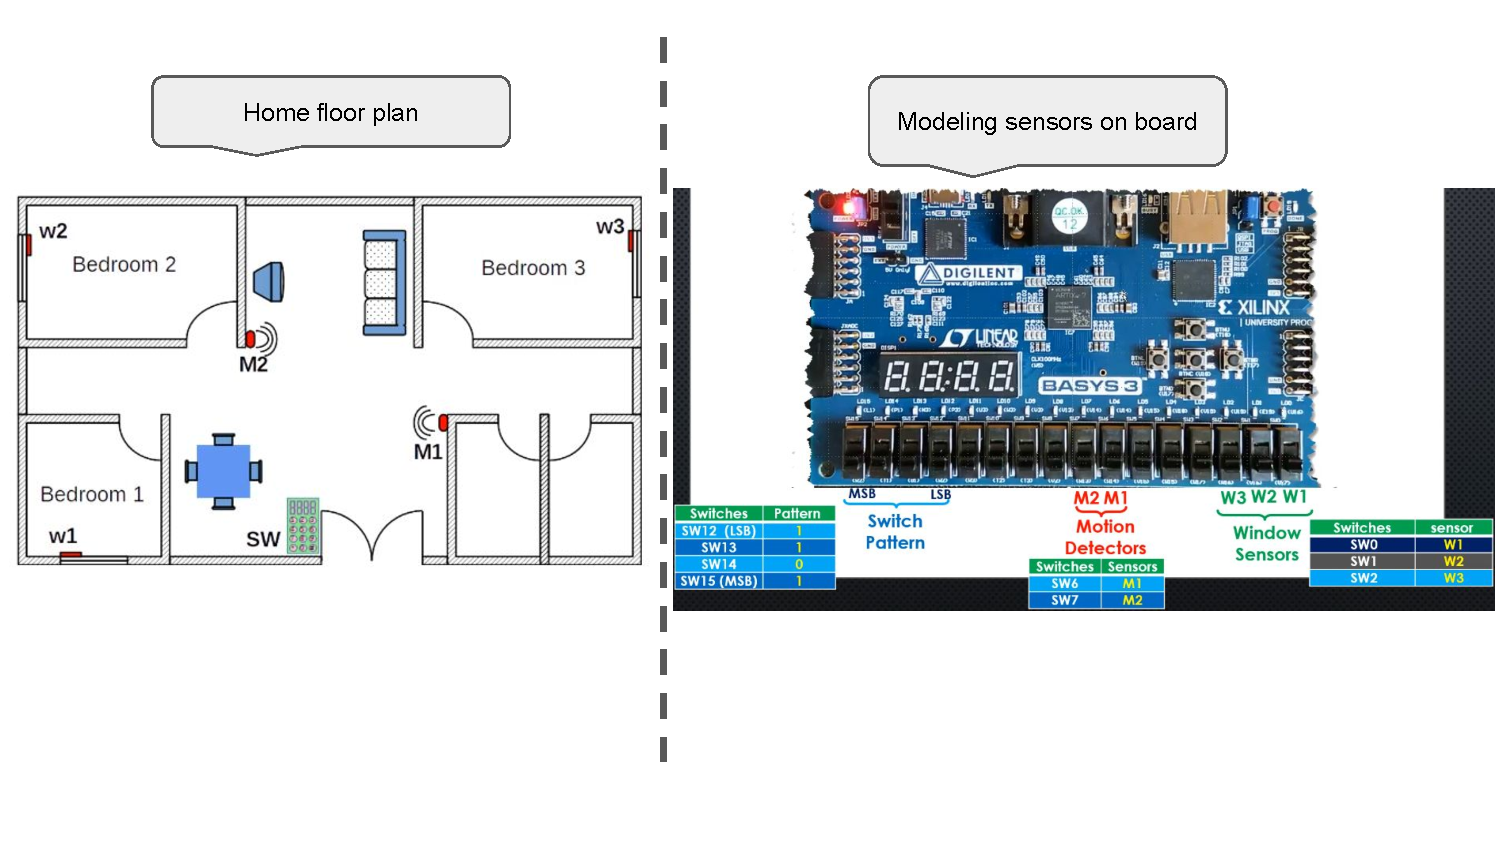
\includegraphics[scale=0.6,frame]{Figures/home_alarm/proj_def}
\caption{Home alarm system project definition}
\label{fig:home_alarm:proj_def}
\end{figure}

\begin{itemize}

\item We have 2 sets of sensors: motion and window

\item For the window: it detects the status of the window

	\begin{itemize}
	\item open window $\leftrightarrow$ logic value 1
	
	\item closed window $\leftrightarrow$ logic value 0

	\end{itemize}

\item For the motion: 1 for motion and 0 for absence of motion

\item The system (that is the set of sensors) is controlled by a control pannel

	\begin{itemize}
	\item It is activated by a pattern of 4 bit: 1101
	\end{itemize}

\item The right column of \autoref{fig:home_alarm:proj_def} contains the switch mapping to model the sensors(window and motion), and also switches for the control pannel

\end{itemize}


The different type of switches will be readed using a 16 bit variable.

\begin{figure}[h]
\centering
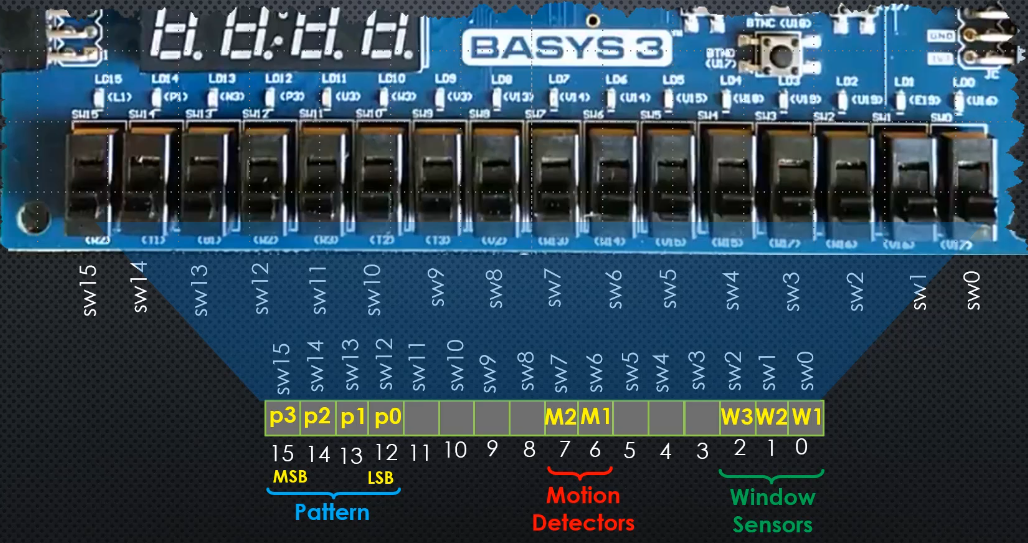
\includegraphics[scale=0.4,frame]{Figures/home_alarm/var_swtiches}
\caption{Switches Variable}
\label{fig:home_alarm:var_swtiches}
\end{figure}

\newpage
\subsection{System Status}
\label{sub:sys_stat}

To get a read for the status of the system, a 7-segement is used. The different cases for system are as follows:

\begin{itemize}

\item \autoref{tab:sys_status} contains 3 cases: system is OFF, ON and no problem is detected, and in case the sensor detects a malfunction.

\begin{table}[h]
\centering
\begin{tabular}{|c|c|}
\hline
System Status & 7-Seg Output \\
\hline
OFF & 0 \\
\hline
ON , no problem & A \\
\hline
Malfunction & E \\
\hline
\end{tabular}
\caption{System Status}
\label{tab:sys_status}
\end{table}

\item Other cases are shown in \autoref{fig:home_alarm:sys_stat_7_seg}.

\begin{figure}[h]
\centering
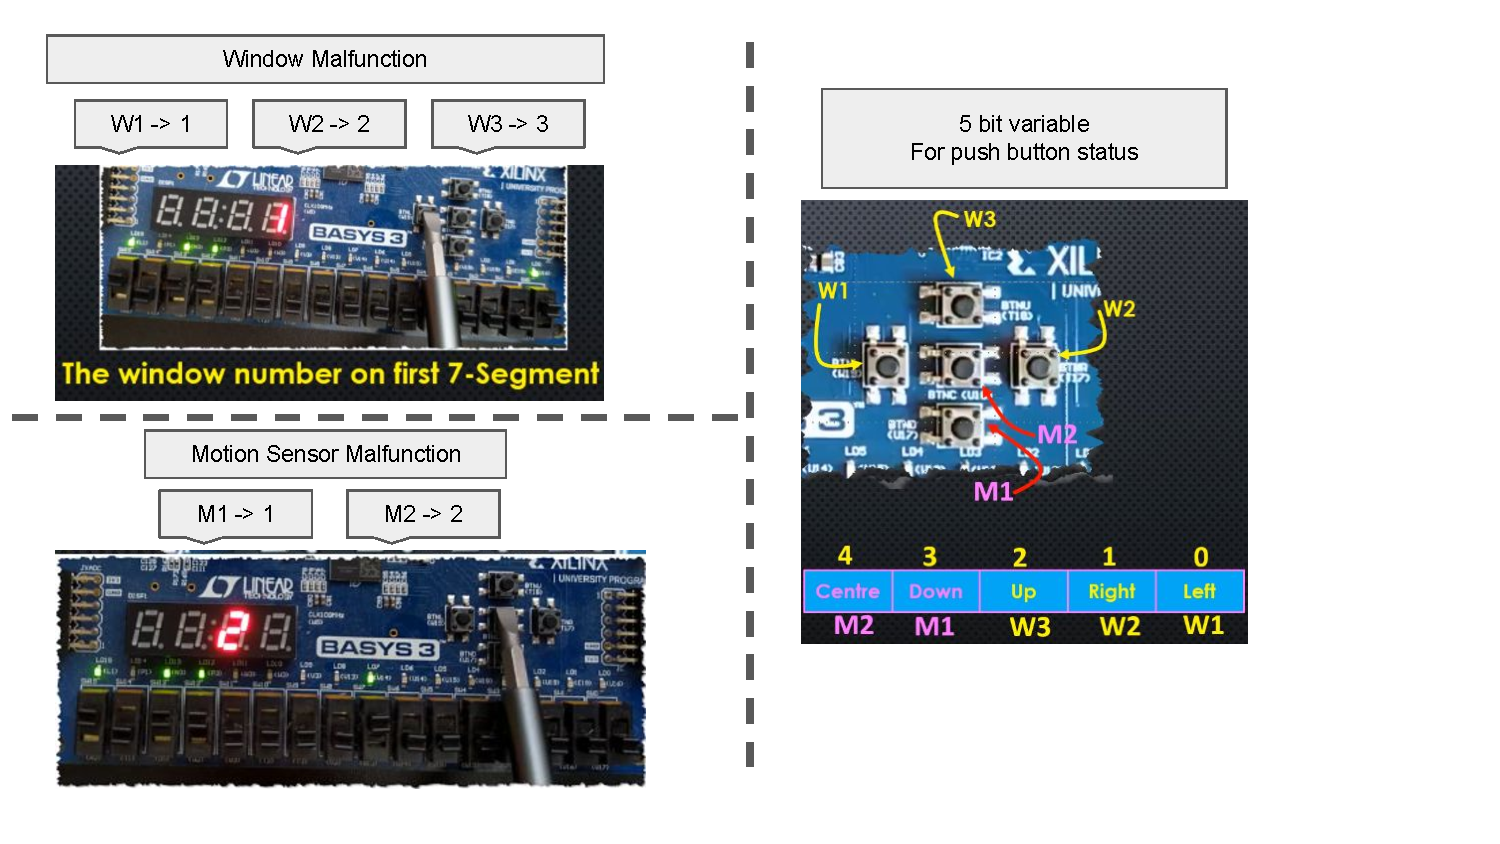
\includegraphics[scale=0.65,frame]{Figures/home_alarm/sys_stat_7_seg}
\caption{Other cases}
\label{fig:home_alarm:sys_stat_7_seg}
\end{figure}

\begin{itemize}
\item For window malfunction: $\mathrm{1}^\mathrm{st}$ digit of 7-seg is used, and motion sensor malfunction: $\mathrm{2}^\mathrm{nd}$ digit

\item Number of window or number of motion sensor is displayed  in each appropriate digit, using corresponding push button. 

\item Finally, a 5 bit variable is used to read the push button status

\end{itemize}


\end{itemize}


\newpage
\section{Code Structure}

\autoref{fig:home_alarm:code_struct} presents the code structure for the alarm system.

\begin{figure}[h]
\centering
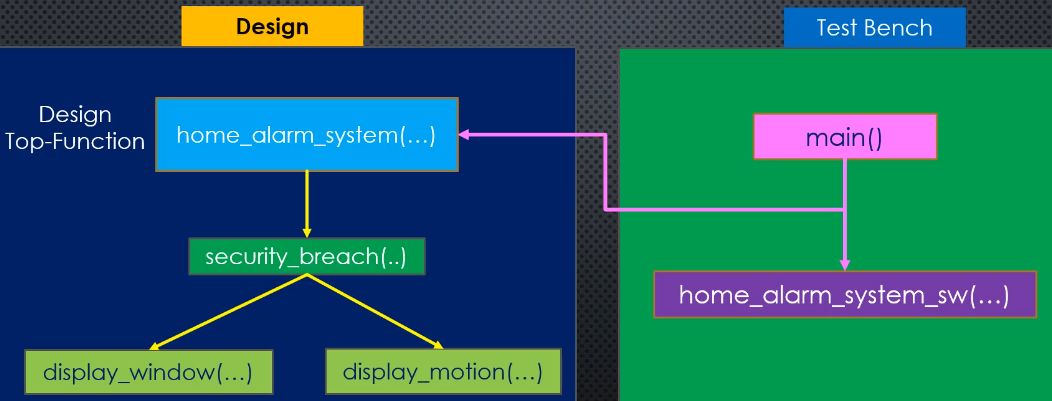
\includegraphics[scale=0.4,frame]{Figures/home_alarm/code_struct}
\caption{Code structure for alarm system}
\label{fig:home_alarm:code_struct}
\end{figure}

\begin{itemize}

\item \verb|home_alarm_system()| is the top function, where it checks all security breach, 
and send proper information for the display pannel.

\item 2 separate sub-function help to send window and motion information to the 7-segment display.

\item Finally a testbench to test the desing behaviour.	

\end{itemize}


\subsection{home-alarm-system()}

\underline{Input Output Arguments:}\\

It receives 2 group of inputs (\verb|silde_switches| and \verb|push_buttons|), and generate 3 group of outputs as shown in \autoref{fig:home_alarm:top_func}.

\begin{figure}[h]
\centering
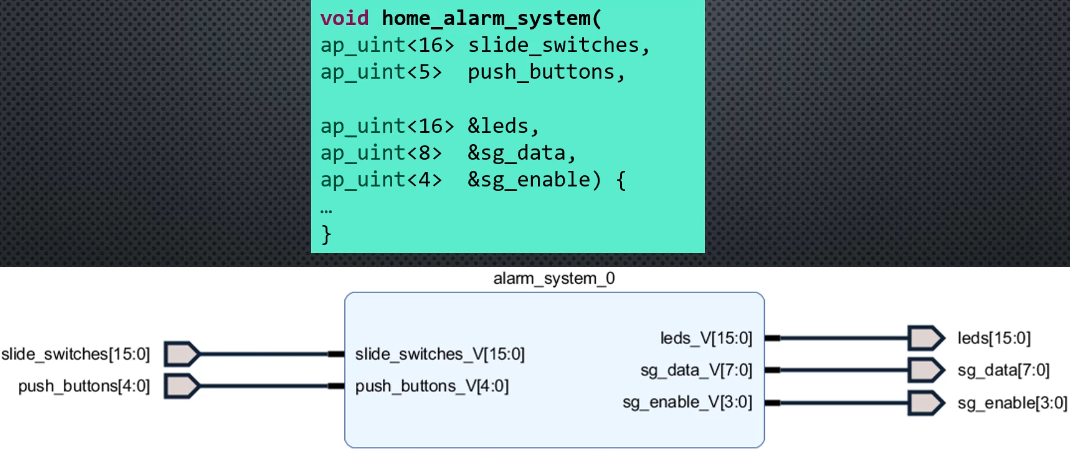
\includegraphics[scale=0.4,frame]{Figures/home_alarm/top_func}
\caption{home-alarm-system() arguments}
\label{fig:home_alarm:top_func}
\end{figure}

\newpage
As a note for the input part:

\begin{itemize}

\item \verb|silde_switches| are normal input as seen in \ref{sub:sys_descrip}.

\item \verb|push_buttons| are for fault detection, that is detect if there is some malfunction as seen in \ref{sub:sys_stat}.

\end{itemize}


The 7-segment code is defined in array as shown in \autoref{fig:home_alarm:7_seg_code_arr}, to extract the correct code and display the associated output at the 7 seg (see \autoref{sec:digit_codes}).

\begin{figure}[h]
\centering
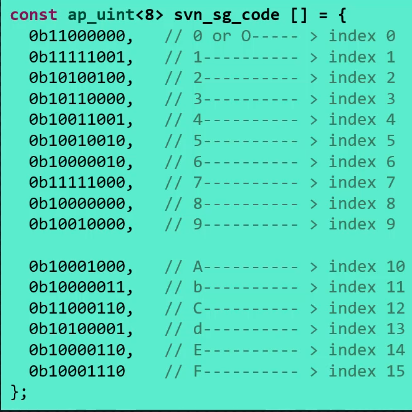
\includegraphics[scale=0.4,frame]{Figures/home_alarm/7_seg_code_arr}
\caption{7-segment code}
\label{fig:home_alarm:7_seg_code_arr}
\end{figure}

\underline{Variable Orgnisation:}\\

Recall from \ref{sub:sys_descrip} (see \autoref{fig:home_alarm:var_swtiches}) that variable switches are stored in a 16 bit variable. \autoref{fig:home_alarm:top_func_steps} contains some of the steps done in the top function:

\begin{figure}[h]
\centering
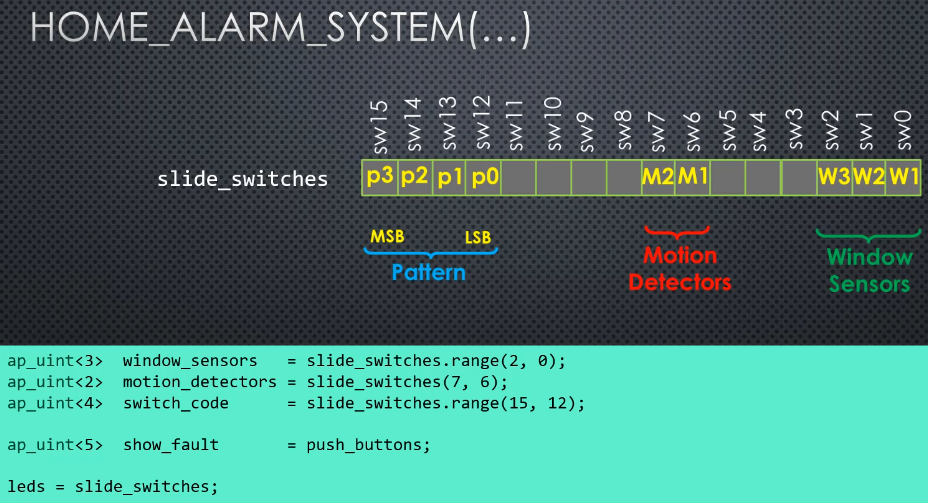
\includegraphics[scale=0.4,frame]{Figures/home_alarm/top_func_steps}
\caption{Top function steps}
\label{fig:home_alarm:top_func_steps}
\end{figure}

\begin{itemize}

\item split the 16 bit \verb|slide_switches| variable into a set of variables

\item stores the \verb|push_buttons| variable into a more descriptive name

\item connect the \verb|slide_switches| directly to the LED

\end{itemize}

\newpage

\underline{System Checking:}\\

\autoref{fig:home_alarm:top_func_checking} shows the checking done.

\begin{figure}[h]
\centering
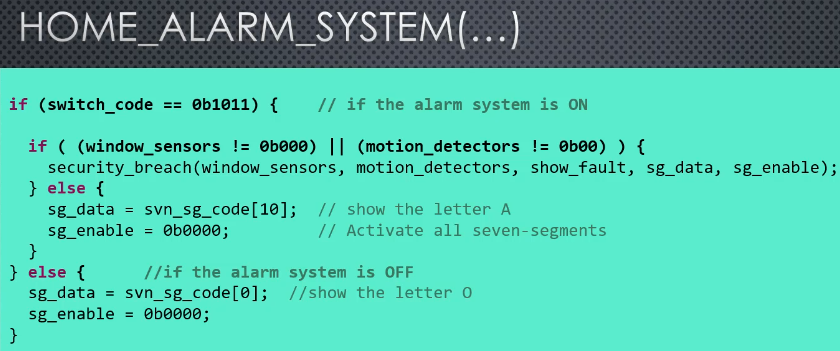
\includegraphics[scale=0.4,frame]{Figures/home_alarm/top_func_checking}
\caption{Top function checking}
\label{fig:home_alarm:top_func_checking}
\end{figure}

\begin{itemize}

\item We check $\mathrm{1}^\mathrm{st}$ the status of the system via the code of the control pannel 

$\leftrightarrow$ \verb|switch_code == 0b1011|

\item If the system is ON,we check for the window and motion sensors

\item if there is not problem, lettre \verb|A| is displayed at the 7 seg (as seen in \autoref{tab:sys_status})

\item If there is a problem, we call \verb|security_breach()| 

\end{itemize}

\subsection{security-breach()}

Now we start by the $\mathrm{2}^\mathrm{nd}$ function \verb|security_breach()|.

\begin{figure}[h]
\centering
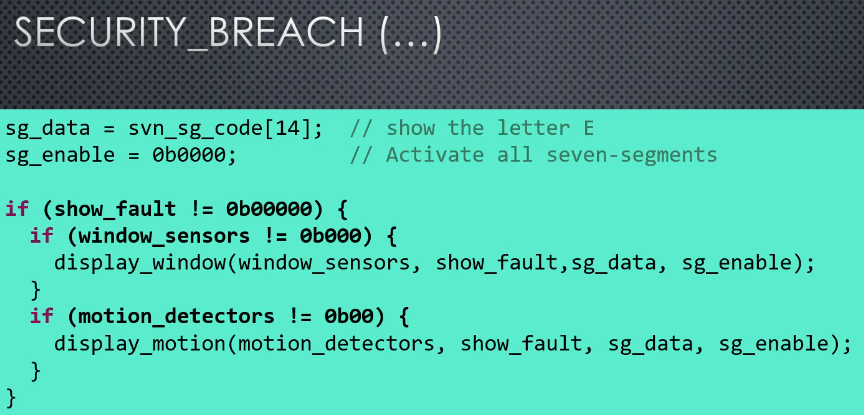
\includegraphics[scale=0.4,frame]{Figures/home_alarm/security_breach_fun}
\caption{security-breach() code}
\label{fig:home_alarm:security_breach_fun}
\end{figure}

\begin{itemize}

\item Initially, it sends the lettre \verb|E| to all 7-seg display.

\item If any of the push button is pressed, $\leftrightarrow$ \verb|show_fault != 0b00000|

it checks if we have an error on the window or motion sensor side.

\end{itemize}


\subsection{diplay-window() and display-motion()}

Functions \verb|diplay_window()| and \verb|display_motion()| are shown in \autoref{fig:home_alarm:disp_win_mot_fun}.


\begin{figure}[h]
\centering
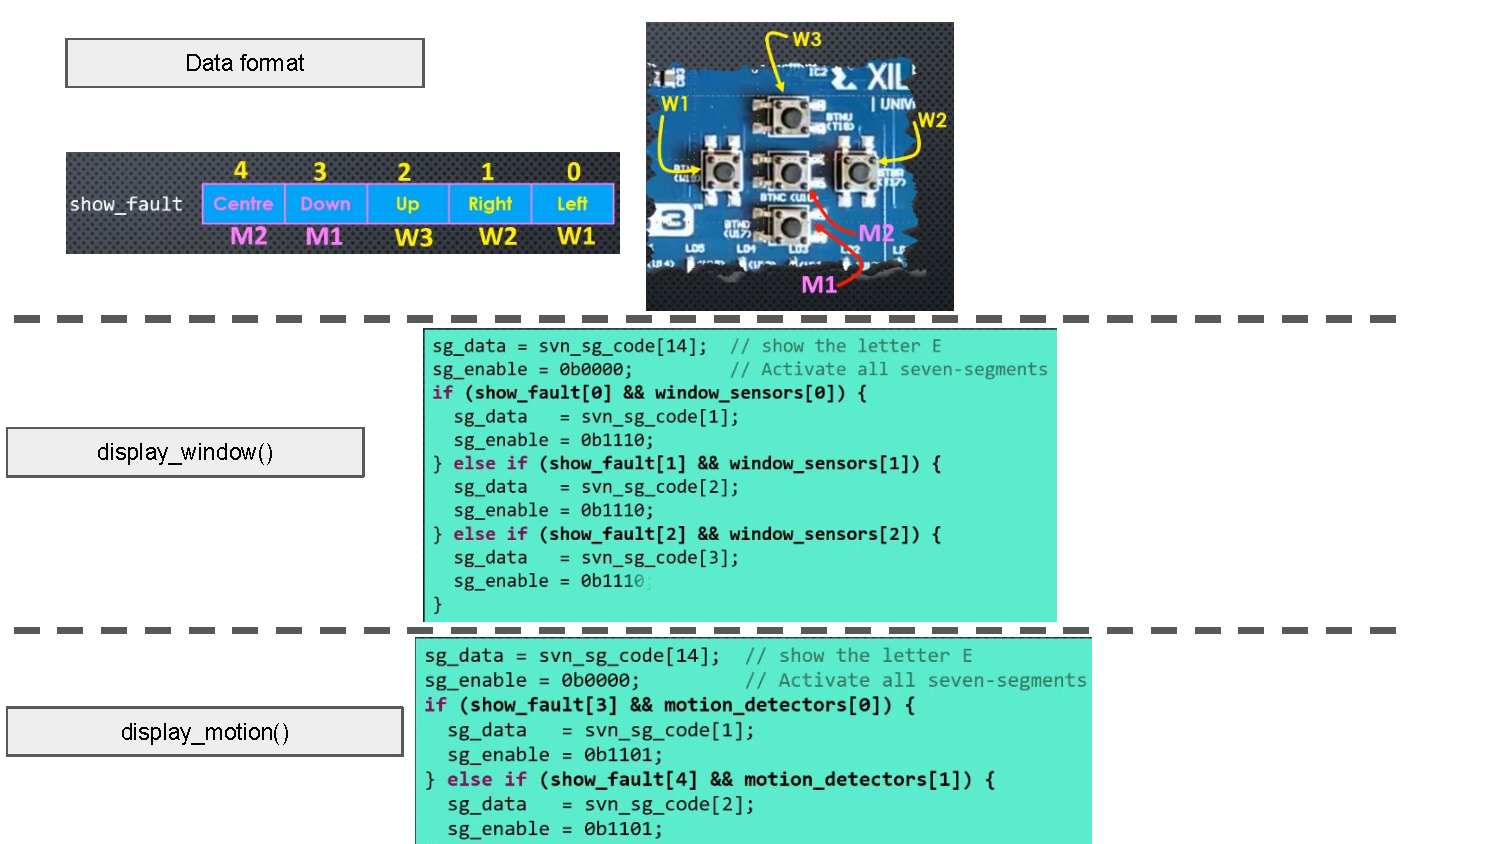
\includegraphics[scale=0.65,frame]{Figures/home_alarm/disp_win_mot_fun}
\caption{diplay-window() and display-motion() code}
\label{fig:home_alarm:disp_win_mot_fun}
\end{figure}

\begin{itemize}

\item In both function, lettre \verb|E| is again displayed into the 7 seg, so we can ensure that the data path is initialized correctly in all part of the \verb|HLS| code

	\begin{itemize}
	\item Otherwise, if we only initialize it using \verb|security_breach()|, the \verb|HLS| tool may use previous value and synthesis some flip flops elements, and the resulting circuit is no combinational anymore.
	\end{itemize}

	

\end{itemize}





